In this chapter we come to the core of this thesis, namely the empirical performance investigation of the Fribourg construction. We are interested in two things. First, how the different versions of the Fribourg construction compare to each other. That is, which combination of optimisations makes the Fribourg construction most efficient? Second, we want to know how the Fribourg construction peforms compared to other complementation constructions. Throughout this thesis, we will refer to the first question as the \textit{internal} investigations, and to the second question as the \textit{external} investigations.

To do an empirical performance investigation we need an implementation of the Fribourg construction. We decided to create this implementation as a part of an existing \om-automata tool called \goal\footnote{\url{http://goal.im.ntu.edu.tw/}}. This tool already contains implementations of various Büchi complementation constructions, so that once our own implementation of the Fribourg construction is in place, we can easily compare it to other constructions (that is, performing the external tests).

Next, we need test data. That is, a set of automata on which to the different complementation constructions. We defined two, very different, test sets. One contains a large number of randomly generated automata and is referred to as the \goal{} test set, and the other contains a very small number of very special automata and is referred to as the Michel test set.

Finally, the experiments need to be executed. Since the complementation of all the automata in our test set with many different constructions is a rather heavy computation task, we decided to make use of a professional high-performance computing (HPC) environment. All the experiments have been carried out on the computer cluster UBELIX at the University of Bern\footnote{\url{http://ubelix.unibe.ch}}.

In this chapter, we are going to describe each of these points in separate sections. Section~\ref{4_exp_setup} also includes our concrete experimental setup, where we present which constructions we are executing for which test data, and what are the allocated resources and imposed constraints. The results of the experiments will finally be presented in Chapter~\ref{chap_results}.


\section{Implementation}



\subsection{GOAL}
\label{4_goal}
\goal{} stands for \textit{Graphical Tool for Omega-Automata and Logics} and is being developed since 2007 at the National Taiwan University (NTU), Department of Information Management\footnote{\url{http://exp.management.ntu.edu.tw/en/IM}}. It has been presented in various scientific publications~\cite{2007_goal}\cite{2008_goal_ext}\cite{2009_goal}\cite{2013_goal}. The tool is freely available on the website \url{http://goal.im.ntu.edu.tw}. It is a Java program, and thus works on all platforms that have a Java runtime environment.\footnote{The required version of the runtime environment is 6 or higher (Java 1.6).}

\goal{} allows to graphically and interactively create and manipulate different types of \om-automata, including non-deterministic Büchi automata. The palette of provided manipulations is vast and ranges from input testing, over conversions to other types of non-deterministic \om-automata, to implementations of graph layout algorithms. Figure~\ref{goal_gui} shows a screenshot of \goal's graphical user interface with an open menu showing the breadth of possible manipulations for \om-automata. 

\begin{figure}[htb!]
\centering
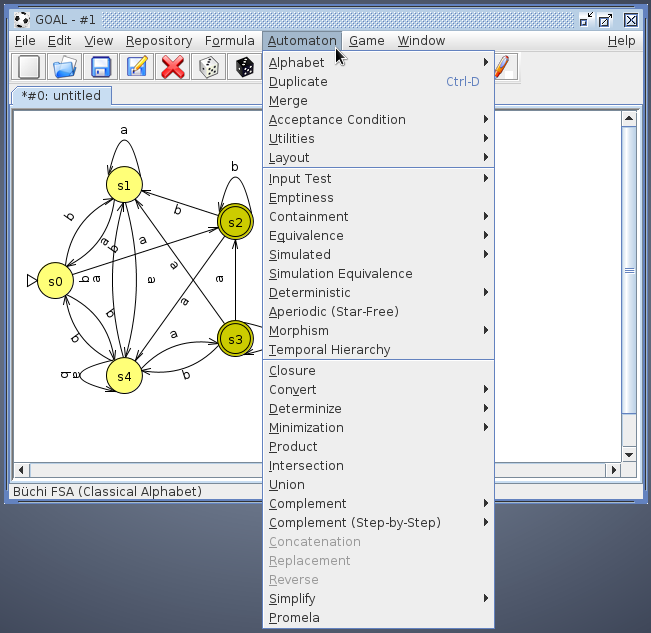
\includegraphics[width=0.4\textwidth]{figures/goal.png}
\caption{The graphical user interface of \goal{} (here version 2014--11--17, which is, at the time of this writing the latest one) with a non-deterministic Büchi automaton in the editor window and an open menu showing the different types of manipulations that are provided for \om-automata.}
\label{goal_gui}
\end{figure}

Relevant for our purposes are the complementation constructions for non-deterministic Büchi automata that \goal{} provides. Also here, \goal{} comes up with a comprehensive offer. In the 2014-11-17 version of \goal{}, there are 10 pre-implemented complementation constructions for NBW. Table~\ref{goal_constructions} summarises these constructions and indicates the authors and the publications on which the implementations are based.

\begin{table}[htb!]
\centering
\begin{tabular}{rlllr}
\hline
\# & Identifier & Name/description & Authors (year) & Ref. \\
\hline
1 & Ramsey & Ramsey-based construction & Sistla, Vardi, Wolper (1987) & \cite{PrasadSistla1987217} \\
2 & Safra & Safra construction & Safra (1988) & \cite{1988_safra_1} \\
3 & ModifiedSafra & Modification by Althoff & Althoff (2006) & \cite{2006_althoff} \\
4 & Piterman & Safra-Piterman construction & Piterman (2007) & \cite{2007_piterman} \\
5 & MS & Muller-Schupp construction & Muller, Schupp (1995) & \cite{Muller199569} \\
6 & Rank & Rank-based construction & Schewe (2009) & \cite{schewe2009buchi} \\
7 & WAPA & Via weak alternating parity automata & Thomas (1999) & \cite{1999_thomas} \\
8 & WAA & Via weak alternating automata & Kupferman, Vardi (2001) & \cite{Kupferman:2001} \\
9 & Slice+P & Slice-based construction (earlier) & Vardi, Wilke (2007) & \cite{vardi2007automata} \\
10 & Slice & Slice-based construction (later) & Kähler, Wilke (2008) & \cite{2008_kaehler} \\
\hline
\end{tabular}
\caption{The pre-implemented NBW complementation constructions in \goal{} (version 2014-11-17).}
\label{goal_constructions}
\end{table}

The construction in Table~\ref{goal_constructions} are sorted by the four fundamental complementation approaches. The first one, Ramsey, is the only construction belonging to the Ramsey-based complementation approach. The following four constructions, Safra, ModifiedSafra, Piterman, and MS, belong to the determinization-based approach. Rank, WAPA, and WAA are representants of the Rank-based approach. Finally, Slice and Slice+P belong to the slice-based approach.

Slice and Slice+P are combined in a single construction in \goal{} but the two specific constructions can be selected by the means of an option. If the P option of Slice is activated, then the Slice+P construction is used, and otherwise the Slice construction is used. In our experiments, we will use the Slice+P version, hoever, we will still refer to this construction as simply Slice in its short form.

Almost the entire functionality of \goal{} is also available via a command line interface. This makes it suitable for automatic batch operation, as it is needed for our experiments. For storing automata, \goal{} defines its own file format called GFF (\goal{} file format) which is based on XML and is typically used with the filename extension \textsf{.gff}.

At this point, it is worth pointing at a related project of the same research group, called the Büchi Store. This is an online repository of classified and tagged \om-automata that can be downloaded in different formats (including GFF). The Büchi Store is located on \url{http://buchi.im.ntu.edu.tw/} and has also been described in a scientific publication~\cite{2011_buchi_store}. Furthermore, there is a binding in \goal{} to the Büchi Store, so that the contents of the store can be directly accessed from \goal{}. For our project we did not make use the Büchi Store, but it is might be an interesting option for related projects.

% GOAL stands for Graphical Tool for Omega-Automata and Logics and has been developed at the National University of Taiwan since 2007~\cite{2007_goal,2008_goal_ext}. The tool is based on the three pillars, \om-automata, temporal logic formulas, and games. It allows to create instances of each of these types, and manipulate them in a multitude of ways. Relevant for our purposes are the \om-automata capabilities of GOAL.

% With GOAL, one can create Büchi, Muller, Rabin, Streett, parity, generalised Büchi, and co-Büchi automata, either by manually defining them, or by having them randomly generated. It is then possible to perform a plethora of operations on these automata. The entirety of provided operations are too many to list, but they include containment testing, equivalence testing, minimisation, determinisation, conversions to other \om-automata types, product, intersection, and, of course, complementation.

% All this is accessible by both, a graphical and a command line interface. The graphical interface is shown in Figure~\ref{goal_gui}. Automata are displayed in the main editor window of the GUI. They can be freely edited, such as adding or removing states and transitions, and arranging the layout. There are also various layout algorithms for automatically laying out large automata. Most of the functionality provided by the graphical interface is also accessible via a command line mode. This makes it suitable for automating the execution of operations.

% \begin{figure}
% \begin{center}
% 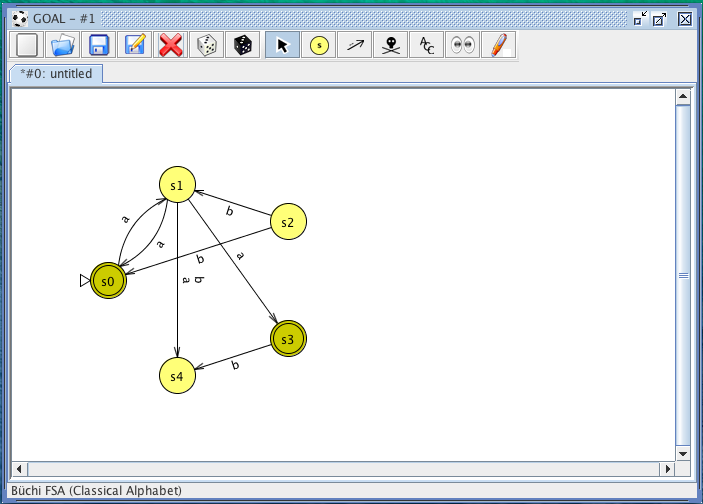
\includegraphics[scale=0.5]{figures/goal_gui.png}
% \caption{Graphical interface of GOAL.}
% \label{goal_gui}
% \end{center}
% \end{figure} 

% For storing automata, GOAL defines an own XML-based file format, called GOAL File Format, usually indicated by the file extension gff.

% An important design concept of GOAL is modularity. GOAL uses the Java Plugin Framework (JPF)~\footnote{http://jpf.sourceforge.net/}, a library for building modular and extensible Java applications. A JPF application defines so-called extension points for which extensions are provided. These extensions contain the actual functionality of the application. Extensions and extension points are bundled in plugins, the main building block of a JPF application. It is therefore possible to extend an existing JPF application by bundling a couple of new extensions for existing extensions points in a new plugin, and installing this plugin into the existing application. On the next start of the application, the new functionality will be included, all without requiring to recompile the existing application or to even have its source code.

% GOAL provides a couple of extensions points, such as \textit{Codec}, \textit{Layout}, or \textit{Complementation Construction}. An extension for \textit{Codec}, for example, allows to add the handling of a new file format which GOAL can read from and write to. With an extension for \textit{Layout} one can add a new layout algorithm for laying out automata in the graphical interface. And an extension to \textsf{Complementation Construction} allows to add a new complementation construction to GOAL. This is how we added the Fribourg construction to GOAL, as we will further explain in Section~\ref{implementation}.

% There are a couple of Büchi complementation constructions pre-implemented in GOAL. Table~\ref{goal_constructions} summarises them, showing for each one its name on the graphical interface and in the command line mode, and the reference to the paper introducing it. As can be seen, the most important representants of all the four approaches (Ramsey-based, determinisation-based, rank-based, and slice-based, see Chapter~\ref{background}) are present. In addition to the listed constructions, GOAL also contains Kurshan's construction and classic complementation. These are for complementing DBW and NFA/DFA, respectively, and thus not relevant to us.

% One of the constructions can be set as the default complementation construction. It is then possible to invoke this construction with the shortcut Ctrl-Alt-C. Furthermore, the default complementation constructions will be used for the containment and equivalence operations on Büchi automata, as they include complementation.

% Complementation constructions in GOAL can define a set of options that can be set by the user. In the graphical interface this is done at the start of the operations via a dialog window, in the command line mode the options are specified as command line arguments. Figure~\ref{goal_complementation_options} shows the options dialog of the Safra-Piterman construction. Complementation options allow to play with different configurations and variants of a construction, and we will make use of them for including the optimisations presented in Chapter~\ref{fribourg_construction} to our implementation of the Fribourg construction.


% \begin{figure}
% \begin{center}
% 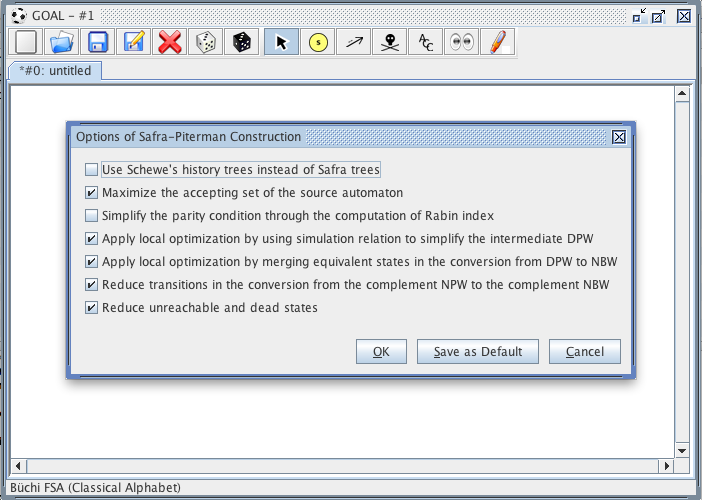
\includegraphics[scale=0.5]{figures/goal_complementation_options.png}
% \caption{Complementation constructions in GOAL can have a set user-selectable options. Here the options of the Safra-Piterman construction.}
% \label{goal_complementation_options}
% \end{center}
% \end{figure}

% For most complementation constructions (all listed in Table~\ref{goal_constructions} except the Ramsey-based construction) there is also a version for step-by-step execution. In this case, the constructions define so-called steps and stages, through which the user can iterate independently. This is a great way for understanding how a complementation construction works, and for investigating specific cases in order to potentially further improve the construction. 


\subsection{Implementation of the Construction}
\label{4_implementation}

\subsubsection{The Extensible Plugin Architecture of \goal}
\goal{} has been designed from the ground up to be modular and extensible. To this end, it has been created with the Java Plugin Framework (JPF)\footnote{\url{http://jpf.sourceforge.net/}}. This framework allows to build applications whose functionality can be easily and seamlessly extended by writing additional plugins for it. These plugins can be installed in the main application without the need to recompile the whole application. Rather, the plugin is compiled separately and the resulting bytecode files are copied to the directory tree of the main application. It is not even necessary to know the source code of the main application in order to write a plugin. The interfaces of JPF itself, and the documentations of the relevant classes of the main application are all that a plugin writer needs to know.

In some more detail, JPF requires an application to define so called extension points. For a given extension point, multiple extensions can be provided. These extensions contain the actual functionality of the application. A JPF application basically consists of a groups of different types of extensions that are plugged in their corresponding extension points. A plugin, finally, is an arbitrary bundle of extensions and extension points. It is the basic unit of organisation in the Java Plugin Framework.

One of the extension points of \goal{} is called is called \textsf{Complementation Construction}. In order to add a new complementation construction to \goal, one has to write an extension for \textsf{Complementation Construction} that contains the implementation of the new construction. This extension can then be bundled as a plugin, and the plugin can be compiled and installed in the main application. This makes the new extension an integral part of the main application. That means that after starting \goal{} with the installed plugin, the new complementation construction is included in \goal{} in exactly the same way as all the other existing complementation constructions are included.

This is exactly what we did in order to add the Fribourg construction to \goal. The name of our plugin is \textsf{ch.unifr.goal.complement}\footnote{By convention, JPF plugins are named after the base package name of their implementation files.} and it is publicly available. Appendix~\ref{app_plugin} contains instructions how the plugin can be obtained and installed.

There is more than just the extension point \textsf{Complementation Construction} that can be extended to add a new complementation construction to \goal. There are separate extension points for including the construction in the command line interface of \goal{}, in the menu structure, or for providing a step-by-step version of the construction. We aimed at making this integration as complete as possible so that the Fribourg construction provides the same facilities as the pre-implemented constructions. This includes, for example, comand line integration (of course required for our experiments), menu integration for setting default options or defining the Fribourg construction as the default complementation construction of \goal, or an interactive step-by-step execution environment.


\subsubsection{The Fribourg Construction Plugin}
In our implementation of the Fribourg construction we also included the three optimisations, R2C, M1, and M2, described in Section~\ref{3_optimisations}. To leave the choice of which optimisations to use for any given complementation task to the user, we implemented these optmisation as \textit{options}. Complementation construction options in the \goal{} GUI are presented to the user as a list of checkboxes immediately before the start of the complementation. The user can then make his or her selection and launch the complementation process. In the command line interface, options are represented as flags that can be added to the corresponding command.

In addition to the three optimisations, we also added further options to our implementation. Table~\ref{goal_options} shows a list of all the available options for the Fribourg construction in the current version of the plugin.


\begin{table}
\centering
\begin{tabular}{ll}
\hline
Identifier & Description \\
\hline
R2C & Deleting states with rightmost colour 2, if automaton is complete \\
M1 & Component merging optimisation \\
M2 & Single 2-coloured component optimisation \\
C & Make input automaton complete \\
R & Remove unreachable and dead states from output automaton \\
RR & Remove unreachable and dead states from input automaton \\
MACC & Maximise accepting states of input automaton \\
B & Use the ``bracket notation'' for state labels \\
\hline
\end{tabular}
\caption{The options of the Fribourg construction in \goal.}
\label{goal_options}
\end{table}

Table~\ref{goal_options} defines an identifier for each option, and we will use these identifiers throughout the rest of this thesis for referring to the corresponding options. These identifiers also correspond to the names of the option flags in the command line interface (in lower case).

The first three options in Table~\ref{goal_options} represent the three optimisations from Section~\ref{3_optimisations}. The R2C optmisation is implemented so that it applies only to input automata that are complete. That is, selecting R2C for the complementation of an automaton that is not complete has no effect, and results in the same as not selecting R2C in the first place.

The options M1 and M2 implement the M1 and M2 optimisations. Since M2 is dependent on M1, we enforced that M2 can only be selected if M1 is also selected.

The C option is one of the option that preprocesses the input automaton before the actual complementation starts. This option checks if the input automaton is complete, that is, if every state has at least one outgoing transition for every symbol of the alphabet. If this is not the case, it makes the automaton complete by adding a sink state. A sink state is a non-accepting state that ``aggregates'' all the missing transitions of incomplete states, so that these states become complete. The sink state itself has transitions to itself for all symbols of the alphabet. The purpose of this option is to be used together with R2C. By making an automaton complete with C, we can ensure that the R2C optimisation will be applied. However, in this case, the size of the automaton to complement is increased by one what is in turn negative for the performance of the construction. This effects has been investigated by Göttel in previous work on the Fribourg construction~\cite{2013_bsc_goettel}, and we will re-investigate hem in this thesis as explained in Section~\ref{4_exp_setup}.

The R option affects the complement automaton after the termination of the construction. Its effect is to remove all the unreachable and dead states from the complement. Unreachable states are states that cannot be reached from the initial state. Dead states are states from which it is not possible to reach an accepting state. These states can be removed from any automaton without changing the language of the automaton. The R option is common among the pre-implemented complementation constructions of \goal. Ramsey, Piterman, Rank, and Slice, all have the R option. It allows for example to determine the number of unreachable and dead state that a complementation construction produces. To this end one can complement the same automaton with and without R and then calculate the difference of the sizes of the two output automata. Such investigations have been done in~\cite{2011_tsai} for some of the pre-implemented complementation constructions in \goal. In our experiments, we will also use the R option, however our investigations on the unreachable and dead states will not be as in-depth as in~\cite{2011_tsai}.

The RR option is similar to the R option, except that it removes the unreachable and dead states from the input automaton, before the start of the actual complementation construction, rather than from the output automaton. The pre-implemented constructions in \goal{} do not have something like the RR option, and we added it to the Fribourg construction just for our own interest.

MACC is also a pre-processing option. Its effect is to maximise the accepting set of the input Büchi automaton. This means that as many states as possible are made accepting without changing the language of the automaton. This technique is introduced and described in~~\cite{2011_tsai}. In this paper Tsai~et~al. state that a higher ratio of accepting states generally results in smaller complements. A result that we can confirm with our own experimental results that we present in Chapter~\ref{chap_results}. The MACC option is available for the Ramsey, Piterman, Rank, and Slice constructions in \goal. In our experiments we will however not make use of the MACC option.

Finally, the B option has no effect on the construction itself. It just activates the ``bracket notation'' for marking the colours of the sets inside the produced states. This notation corresponds to the notation we used throughout Chapter~\ref{chap_construction}. With the standard notation, sets are represented as 2-tuples, where the first element is the actual set of states and the second element is the colour of the set.



% We implemented the Fribourg construction, including its optimisations, in Java as a plugin for GOAL. This means that after installing out plugin to an existing GOAL installation\footnote{As the plugin interfaces of GOAL have recently changed, the can be used only for GOAL versions 2014-11-17 and newer.}, the Fribourg construction will be an integral part of GOAL and can be used in the same way as any other pre-existing complementation construction.

% To keep the Fribourg construction flexible, we made use of options. The three optimisations described in Section~\ref{optimisations} are presented to the user as selectable options. Additionally, we included several further options. Table~\ref{goal_fribourg_options} lists them all. For convenience, we use for each options a short code name, which is also used as the option name in the command line mode.

% \begin{table}
% \caption{The options for the Fribourg construction.}
% \begin{center}
% \begin{tabular}{|l|l|}
% \hline
% Code & Description \\ \hline
% m1 & Component merging optimisation \\ \hline
% m2 & Single 2-coloured component optimisation \\ \hline
% r2c & Deleting states with rightmost colour 2, if automaton is complete \\ \hline
% c & Make input automaton complete \\ \hline
% macc & Maximise accepting states of input automaton \\ \hline
% r & Remove unreachable and dead states from output automaton \\ \hline
% rr & Remove unreachable and dead states from input automaton \\ \hline
% b & Use the ``bracket notation'' for state labels \\ \hline
% \end{tabular}
% \end{center}
% \label{goal_fribourg_options}
% \end{table}

% The first three items in Table~\ref{goal_fribourg_options}, m1, m2, and r2c, correspond to the optimisations M1, M2, and R2C, described in Section~\ref{optimisations}. As the M2 optimisation requires M1, our implementation makes sure that the m2 option can only be selected if also the m1 option is selected. The \tec{c} option, for making the input automaton complete before starting the actual construction, is intended to be used with the \tec{r2c} option. In this way, the R2C optimisation can be forced to apply. This idea results from previous work that investigated whether making the input automaton complete plus the application of the R2C optimisation brings an improvement over the bare Fribourg constructoin~\cite{2013_bsc_goettel}. The result was negative, that is, the construction performs worse with this variant on practical cases. Also note that using the \tec{c} option alone, very likely decreases the performance of the construction, because the automaton is made bigger if it is not complete.

% The \tec{macc} and \tec{r} options are common among the other complementation constructions in GOAL. The first one, \tec{macc}, maximises the accepting set of the input automaton. That means, it makes as many states accepting as possible without changing the automaton's language. This should help to make the complement automaton smaller. The \tec{r} options prunes unreachable and dead states from the complement automaton. Unreachable states are states that cannot be reached from the initial states, and dead states are states from where no accepting state can be reached. Clearly, all the runs containing an unreachable or dead state are not accepting, and thus these states can be removed from the automaton without changing its language. The complement automaton can in this way be made smaller. The \tec{rr} option in turn removes the unreachable and dead states from the \emph{input} automaton. That is, it makes the input automaton smaller, before the actual construction starts, what theoretically results in smaller complement automaton.

% Finally, the \tec{b} option affects just the display of the state labels of the complement automaton. It uses an alternative notation which uses different kinds of brackets, instead of the explicit colour number, to indicate the colours of sets. In particular, 2-coloured sets are indicated by square brackets, 1-coloured sets by round parenthesis, and 0-coloured sets by curly braces. Sets of states of the upper part of the automaton are enclosed by circumflexes. This notation, although being very informal, has proven to be very convenient during the development of the construction.

% When we developed the plugin, we aimed for a complete as possible integration with GOAL. We integrated the Friboug construction in the graphical, as well as in the command line interface. We added a step-by-step execution of the construction in the graphical interface. We provided that customised option configurations can be persistently saved, and reset to the defaults at any time. We also integrated the Fribourg construction in the GOAL preferences menu so that it can be selected as the default complementation construction. In this way, it can be invoked with a key-shortcut and it will also be used for the containment and equivalence operations. Our goal is that once the plugin is installed, the Fribourg construction is as seamlessly integrated in GOAL as all the other pre-existing complementation construction.

% The complete integration allows us to publish the plugin so that it can be used by other GOAL users. At the time of this writing, the plugin is accessible at \url{http://goal.s3.amazonaws.com/Fribourg.tar.gz} and also over the GOAL website\footnote{http://goal.im.ntu.edu.tw/}. The installation is done by simply extracting the archive file and copying the contained folder to the \tec{plugins/} folder in the GOAL system tree. No compilation is necessary. The same plugin and the same installation procedure works FOR Linux, Mac OS X, Microsoft Windows, and other operating systems that run GOAL.

% Since between the 2014-08-08 and 2014-11-17 releases of GOAL certain parts of the plugin interfaces have changed, and we adapted our plugin accordingly, the currently maintained version of the plugin works only with GOAL versions 2014-11-17 or newer. It is thus essential for any GOAL user to update to this version in order to use our plugin.

\subsection{Verification of the Implementation}
Having an implementation of a complementation construction, one also needs to be sure that this implementation is correct. That is, the language of an output automaton must really be the complement of the language of the input automaton. It is crucial that this is the case, especially when doing empirical performance investigations. A construction that produces wrong results would lead to a misinterpretation of the actual performance of the construction.

In order to verify the correctness of our implementation, we chose to compare the results of our construction to the results of the pre-implemented complementation constructions of \goal. The existing complementation constructions in \goal{} are thus taken as the ``ground truth''. Concretely, the approach is as follows. We take an automaton $A$ and complement it with, say, the Piterman construction in \goal{}. This yields automaton $A^\prime$. Then we complement the same automaton $A$ with the Fribourg construction, what yields automaton $A^{\prime\prime}$. By the means of \goal's equivalence operation, we then test whether $A^\prime$ and $A^{\prime\prime}$ accept the same language. We call this procedure \textit{complement-equivalence test}.

Of course, with such an empirical approach it is not possible to conclusively verify that our implementation of the Fribourg construction is correct. This would require to do a complement-equivalence test for each of an infinite number of automata, which is not possible. With this approach we can only conclusively falsify the correctness of the implementation, as a single counterexample is enough to prove that the implementation produces wrong results. However, we think that the absence of counterexamples for a certain number of cases is still a good indicator that there are no errors in the implementation and thus confirms our hypothesis that the implementation is correct.

Concretely, we did 1,000 complement-equivalence tests for different versions of the Fribourg construction (resulting from different sets of activated options) with random automata. The automata we used for the test had four states, an alphabet size between 2 and 4, and were generated with the random automaton generation operatio of \goal. The concrete versions of the Fribourg construction that we tested are:
\begin{itemize}
\item Fribourg
\item Fribourg+R2C+C
\item Fribourg+M1
\item Fribourg+M1+M2
\item Fribourg+R
\item Fribourg+RR
\item Fribourg+MACC
\end{itemize}
For each of these versions, the 1,000 random test automata have been generated on-the-fly. The used ``ground truth'' construction was Piterman. All of the tests were successful, that is, there were no counterexamples.

The reason that we chose rather small test automata is to avoid practical problems regarding time and memory requirements during the computation. The equivalence operation in \goal{} is implemented as a reciprocal containment test, which includes complementation. For a complement-equivalence test, we thus have to complement the complements of the initial automata. If the initial automata are too big, then their complements might be already so big that it becomes practically infeasible to complement them again.

These tests are certainly not extensive, and it would also be interesting to use larger and more complex automata as test cases (maybe with a different testing approach). However, given the results of the tasts we made, we are still confident that our implemenation is correct with a high probability. 

With the above listing of Fribourg construction versions (for example, Fribourg+R2C+C) we also introduce a notation that we will use throughout the rest of this thesis. The first token is the base construction and is one of the identifiers in Table~\ref{goal_construcions} in Section~\ref{4_goal}. The option identifiers appended with plus signs indicate which options (if any) are ``activated'' in the given version of the construction.

% See UBELIX/jobs/2014-11-25

% Can we do a complement-equivalence test with all the 11,000 automata of size 15 in the test set?

% Of course it is needed to test whether our implementation produces correct results. That is, are the output automata really the complements of the input automata? We chose doing so with an empirical approach, taking one of the pre-existing complementation constructions in GOAL as the ``ground truth''. We can then perform what we call complementation-equivalence tests. We take a random Büchi automaton and complement it with the ground-truth construction. We then complement the same automaton with our implementation of the Fribourg construction, and check whether the two complement automata are equivalent. Provided that the ground-truth construction is correct, we can show in this way that our construction is correct for this specific case.

% We performed complementation-equivalence tests for the Fribourg construction with different option combinations. In particular, we tested the configurations \tec{m1}, \tec{m1}+\tec{m2}, \tec{c}+\tec{r2c}, \tec{macc}, \tec{r}, \tec{rr}, and the construction without any options. For each configuration we tested 1000 random automata of size 4 and with an alphabet of size 2 to 4. As the ground-truth construction we chose the Safra-Piterman construction. In all cases the complement of the Fribourg construction was equivalent to the complement of the Safra-Piterman construction.

% Doubtlessly, it would be desirable to test more, and especially bigger and more diverse automata. However, by doing so one would quickly face practical problems due to long complementation times with bigger automata and larger alphabets, and high memory usage. For our current purpose, however, the tests we did are enough for us to be confident that our implementation is correct.

\section{Test Data}
The core of this thesis is to empirically investigate the performance of the Fribourg construction. To this end, we ``feed'' concrete automata to the Fribourg construction and analyse the results. This set of automata is our3 test data and is of crucial importance for the validity of the performance investigation. Test data should not be biased in favour or unfavour of one of the tested algorithms. Ideally, publicly available, or even standardised, test data is used, that has been previously used in other experiments. Furthermore, test data should cover interesting cases that reveal important aspects about the algorithm.

For our investigation we chose two test sets that are publicly known or available and cover very different scenarios. While one of them consists of 11,000 automata and tries to cover a broad range of ``everyday'' complementation problems, the other one consists of just 4 automata, that are however very special. We call the former one the \goal{} test set and the latter on the Michel test set, and we are going to describe them in the following two sections.


\subsection{GOAL Test Set}
\label{4_goal_testset}

\subsubsection{Introduction}
The \goal{} test set has been created by Tsai~et~al. for the experiments described in the the paper \textit{State of Büchi Complementation}~\cite{2010_tsai}. In this paper, the authors carry out empirical performance investigations of Büchi complementation constructions that are very similar to our own investigations. The experiments were run with the \goal{} tool, hence the name \goal{} test set. The idea leading the design of this test set was to generate a large set of complementation problems with various difficulty levels.

The test set consists of 11,000 automata of size 15, and with an alphabet size of 2. Within the given constraints, the 11,000 automata were generated at random. The test set is furthermore structured into 110 classes that are combinations of two parameters, the so called transition density and the acceptance density. Simply speaking, the transition density determines the number of transitions in an automaton, and the acceptance density determines the number of accepting states.

More precisely, the transition density $t$ is defined as follows. Let $n$ be the number of states of automaton $A$, and $t$ its transition density. Then $A$ contains $tn$ transitions for each symbol of the alphabet\footnote{In the case $tn$ is not an integer, it is rounded up to the next integer.}. That is, if one of our test set automata with 15 states and the alphabet ${0, 1}$ has a transition density of 2, then it contains exactly 30 transtions for symbol $0$ and 30 transitions for symbol $1$. Consequently, each state has on average two outgoing and two incoming transitions for each symbol. Therefore, the transition density can also be seen as the average number of outgoing and incoming transitons per alphabet symbol that a state has.

The acceptance density $a$ is defined as the ratio of accepting states to non-accepting states in the automaton. That is, if automaton $A$ has $n$ states and an acceptance density of $a$, then it contains $an$ accepting states\footnote{Again, if $an$ is not an integer, it is rounded up to the next integer.}. The acceptance density is thus bound to a number between 0 and 1. For example, if an automaton of our test set has an acceptance density of 0.1, then it has 2 accepting states, and if an automaton has an accepting density of 1, then all of its states are accepting states.

In the \goal{} test set there are 11 transiton densities and 10 acceptance densities. The transition densities range from 1 to 3 in steps of 0.2, and the acceptance densities range from 0.1 to 1 in steps of 0.1. Thus, we have
\begin{align*}
t^\prime& = \{ 1.0,\,1.2,\,1.4,\,1.6,\,1.8,\,2.0,\,2.2,\,2.4,\,2.6,\,2.8,\,3.0 \} \\
a^\prime & = \{ 0.1,\,0.2,\,0.3,\,0.4,\,0.5,\,0.6,\,0.7,\,0.8,\,0.9,\,1.0 \}
\end{align*}

The 110 classes result from the Cartesian product of $t^\prime$ and $a^\prime$. Each class consequently contains 100 automata. Throughout this thesis, we will often present these classes as a $11 \times 10$ matrix where the rows represent the transition densities $t^\prime$, and the columns represent the acceptance densities $a^\prime$.

There is a second \goal{} test set that is similar to the one that we just described, except that the automata sizes are 20 instead of 15. Tsai~et~al.~\cite{2010_tsai} did their experiments with both, the size-15 (as the primary), and the size-20 (as the scondary) test set. For our own experiments we we are not using the size-20 test set. First, we think that repeating the experiments with the size-20 test set would add only a limited amount of insight. It might be more beneficial to do further tests with a more diverse type of test data, like for example the Michel test set that we describe in the next section. Furthermore, the bigger automata sizes in the size-20 test set are likely to cause practical problems in terms of computing and time resources (see Section~\ref{4_exec_env}). We decided therefore to restrict ourselves to the size-15 test set, and when we refer to \textit{the} \goal{} test set throughout the rest of this thesis, we specifically mean the size-15 test set.

The \goal{} test sets (both, size-15 and size-20) are publicly available on the \goal{} website via the following link: \url{http://goal.im.ntu.edu.tw/wiki/lib/exe/fetch.php?media=goal:ciaa2010_automata.tar.gz}.

\subsubsection{Analysis}

% Format matrices
\renewcommand{\tabcolsep}{0.05cm}
\renewcommand{\arraystretch}{1.05}
\newcolumntype{R}{>{\raggedleft\arraybackslash}p{1.5em}}
\begin{figure}[htb!]
  \centering
  \begin{subfigure}{\textwidth}
    \begin{subtable}{0.47\textwidth}
    % latex table generated in R 3.1.2 by xtable 1.7-4 package
% Sun Aug 16 12:48:04 2015
\begin{tabular}{r|RRRRRRRRRR}
  & 0.1 & 0.2 & 0.3 & 0.4 & 0.5 & 0.6 & 0.7 & 0.8 & 0.9 & 1.0 \\ 
  \hline
1.0 & 0 & 0 & 0 & 0 & 0 & 0 & 0 & 0 & 0 & 0 \\ 
  1.2 & 0 & 0 & 0 & 0 & 0 & 0 & 0 & 0 & 0 & 0 \\ 
  1.4 & 0 & 0 & 0 & 0 & 0 & 0 & 0 & 0 & 0 & 0 \\ 
  1.6 & 0 & 0 & 0 & 0 & 0 & 0 & 0 & 0 & 0 & 0 \\ 
  1.8 & 1 & 1 & 0 & 0 & 0 & 1 & 1 & 1 & 0 & 0 \\ 
  2.0 & 0 & 5 & 1 & 2 & 2 & 3 & 1 & 2 & 2 & 2 \\ 
  2.2 & 5 & 10 & 8 & 5 & 3 & 5 & 8 & 6 & 7 & 1 \\ 
  2.4 & 10 & 6 & 11 & 11 & 8 & 6 & 10 & 20 & 9 & 7 \\ 
  2.6 & 17 & 17 & 12 & 16 & 14 & 19 & 22 & 21 & 19 & 19 \\ 
  2.8 & 27 & 20 & 29 & 32 & 26 & 27 & 30 & 25 & 24 & 19 \\ 
  3.0 & 37 & 37 & 40 & 39 & 34 & 37 & 38 & 35 & 38 & 39 \\ 
  \end{tabular}

    \end{subtable}
    \hfill
    \begin{subfigure}{0.52\textwidth}
    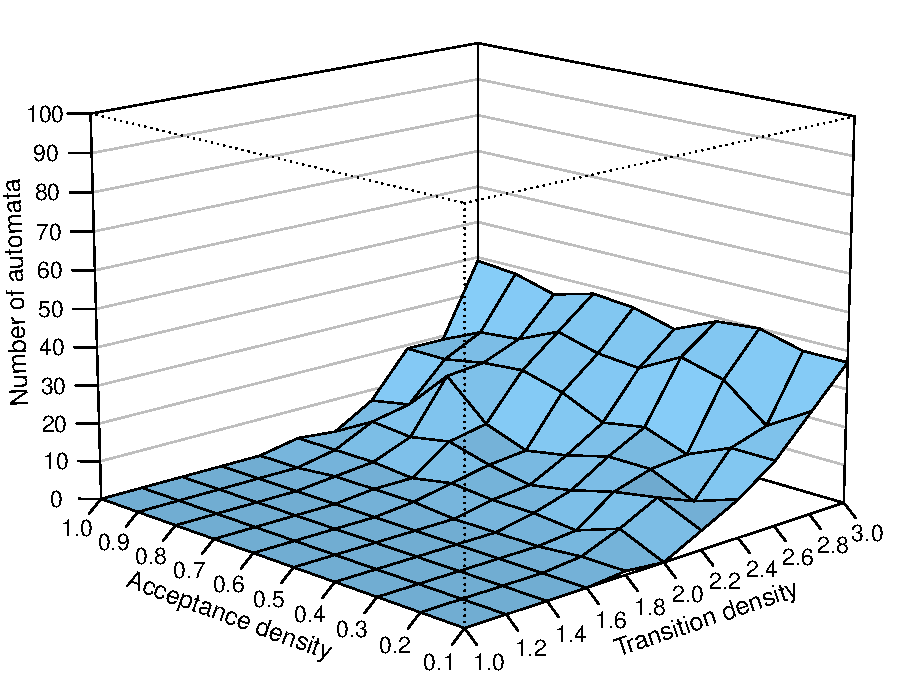
\includegraphics[width=\textwidth]{figures/r/testset/compl.persp.pdf}
    \end{subfigure}
  \caption{Completeness}
  \end{subfigure}

 \begin{subfigure}{\textwidth}
    \begin{subtable}{0.47\textwidth}
    % latex table generated in R 3.1.2 by xtable 1.7-4 package
% Sun Aug 16 12:48:04 2015
\begin{tabular}{r|RRRRRRRRRR}
  & 0.1 & 0.2 & 0.3 & 0.4 & 0.5 & 0.6 & 0.7 & 0.8 & 0.9 & 1.0 \\ 
  \hline
1.0 & 4 & 5 & 5 & 7 & 8 & 4 & 6 & 10 & 4 & 3 \\ 
  1.2 & 1 & 3 & 5 & 8 & 8 & 12 & 10 & 13 & 4 & 14 \\ 
  1.4 & 2 & 17 & 13 & 17 & 20 & 24 & 22 & 21 & 27 & 26 \\ 
  1.6 & 16 & 28 & 30 & 37 & 49 & 42 & 42 & 49 & 45 & 45 \\ 
  1.8 & 31 & 40 & 55 & 59 & 64 & 67 & 76 & 70 & 63 & 78 \\ 
  2.0 & 60 & 64 & 85 & 75 & 83 & 83 & 79 & 90 & 87 & 83 \\ 
  2.2 & 67 & 87 & 86 & 88 & 89 & 91 & 89 & 89 & 89 & 86 \\ 
  2.4 & 88 & 89 & 86 & 92 & 95 & 95 & 94 & 97 & 96 & 97 \\ 
  2.6 & 86 & 93 & 92 & 97 & 97 & 97 & 98 & 96 & 98 & 96 \\ 
  2.8 & 94 & 97 & 95 & 94 & 97 & 99 & 98 & 97 & 97 & 100 \\ 
  3.0 & 99 & 99 & 99 & 97 & 99 & 98 & 100 & 100 & 100 & 99 \\ 
  \end{tabular}

    \end{subtable}
    \hfill
    \begin{subfigure}{0.52\textwidth}
    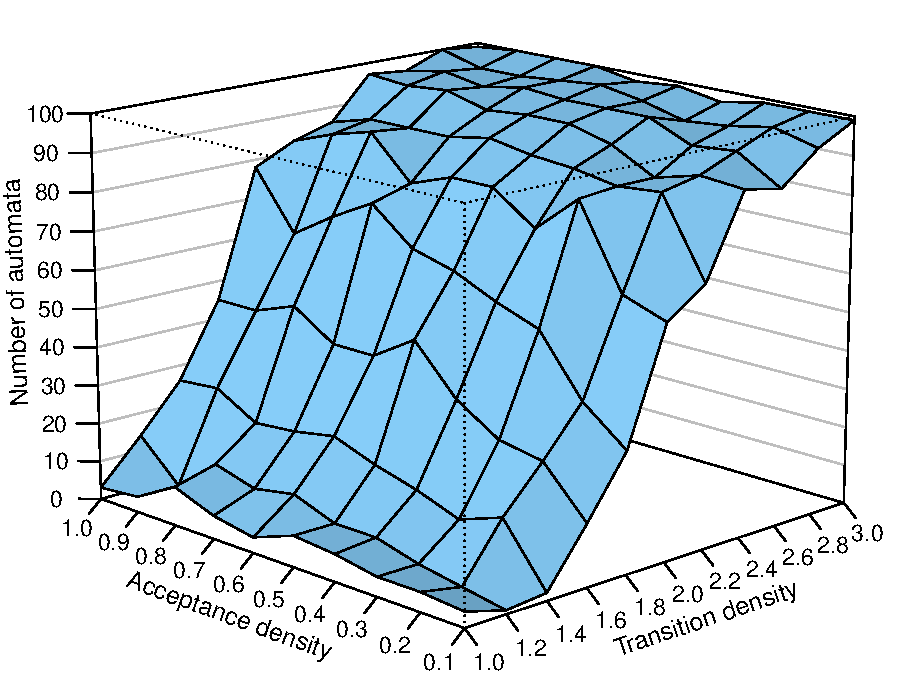
\includegraphics[width=\textwidth]{figures/r/testset/univ.persp.pdf}
    \end{subfigure}
  \caption{Universality}
  \end{subfigure}

  \begin{subfigure}{\textwidth}
    \begin{subtable}{0.47\textwidth}
    % latex table generated in R 3.1.2 by xtable 1.7-4 package
% Sun Aug 16 12:48:05 2015
\begin{tabular}{r|RRRRRRRRRR}
  & 0.1 & 0.2 & 0.3 & 0.4 & 0.5 & 0.6 & 0.7 & 0.8 & 0.9 & 1.0 \\ 
  \hline
1.0 & 17 & 7 & 4 & 5 & 2 & 4 & 3 & 1 & 1 & 0 \\ 
  1.2 & 4 & 2 & 1 & 1 & 0 & 1 & 0 & 0 & 0 & 0 \\ 
  1.4 & 2 & 1 & 0 & 0 & 0 & 0 & 0 & 0 & 1 & 2 \\ 
  1.6 & 0 & 0 & 0 & 0 & 0 & 0 & 1 & 0 & 0 & 0 \\ 
  1.8 & 1 & 0 & 0 & 0 & 1 & 0 & 0 & 0 & 0 & 0 \\ 
  2.0 & 0 & 0 & 0 & 0 & 0 & 0 & 0 & 0 & 0 & 0 \\ 
  2.2 & 0 & 0 & 0 & 0 & 0 & 0 & 0 & 0 & 0 & 0 \\ 
  2.4 & 0 & 0 & 0 & 0 & 0 & 0 & 0 & 0 & 0 & 0 \\ 
  2.6 & 0 & 0 & 0 & 0 & 0 & 0 & 0 & 0 & 0 & 0 \\ 
  2.8 & 0 & 0 & 0 & 0 & 0 & 0 & 0 & 0 & 0 & 0 \\ 
  3.0 & 0 & 0 & 0 & 0 & 0 & 0 & 0 & 0 & 0 & 0 \\ 
  \end{tabular}

    \end{subtable}
    \hfill
    \begin{subfigure}{0.52\textwidth}
    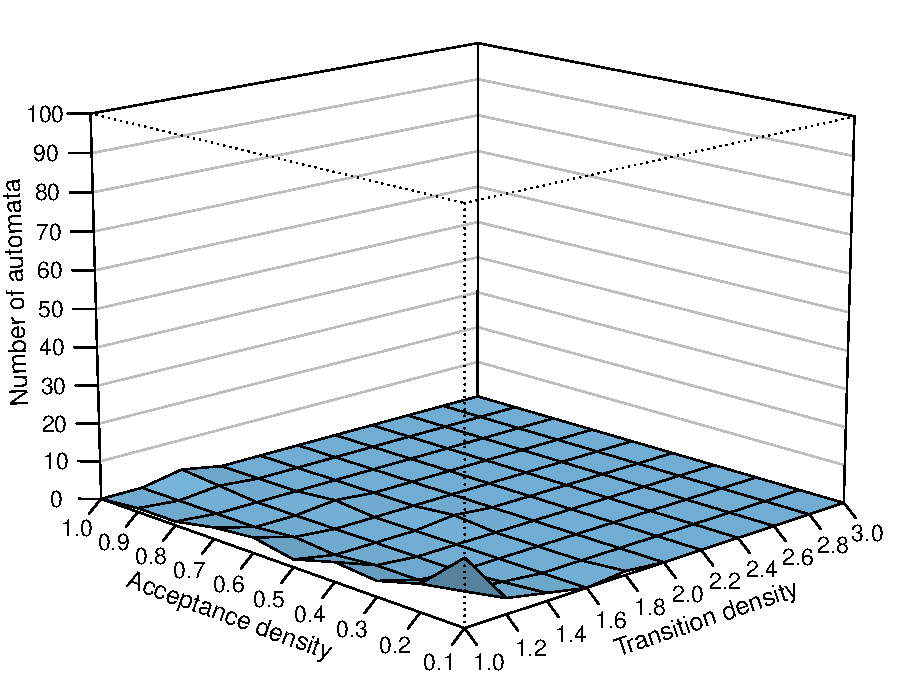
\includegraphics[width=\textwidth]{figures/r/testset/empt.persp.pdf}
    \end{subfigure}
  \caption{Emptiness}
  \end{subfigure}
\caption{Completeness and universality in the GOAL test set.}
\label{4_testset_analysis}
\end{figure}
\tablestyle  % Reset old table style

We analysed some properties of the \goal{} test set that may be of importance for the interpretation of the results of our experiments. In particular, we tested how many automata of the \goal{} test set are \textit{complete}, \textit{universal}, and \textit{empty}.

An automaton is complete if every state has at least one outgoing transition for every symbol of the alphabet. Universality means that an automaton accepts \textit{every} word that can be generated from its alphabet. Emptiness is the contrary of universality and means that an automaton does not accept \textit{any} word (except the empty word $\epsilon$).

To know how many automata are complete is relevant because the R2C optimisation of the Fribourg construction only applies to complete automata. Universality and emptiness are interesting because their respective complement sizes have a lower bound of 1. The complement of a universal automaton is an empty automaton, which can be represented by a single state, and the complement of an empty automaton is a universal automaton which can be represented by a single state as well. In this way we can get an idea of how many unreachable and dead states the Fribourg construction produces. If the produced complement of a universal automata has, say, 2,000 states then 1,999 states of this automata are actually unnecessary as the same automaton could be represented by a single state. We will investigate this aspect to some extent with the R option for the Fribourg construction (see Section~\ref{4_exp_setup}.

\goal{} provides a command for testing emptiness of an automaton. However, it does not provide commands for testing completeness and universality. We therefore implemented these commands on our own as a separate \goal{} plugin (\textsf{ch.unifr.goal.util}, also available as described in Appendix~\ref{app_plugin}). The tests were executed in the execution environment as described in Section~\ref{4_exec_env}. The overall results are as follows.

\begin{itemize}
\item 990 of the 11,000 automata are complete (9\%)
\item 6,796 of the 11,000 automata are universal (61.8\%)
\item 63 of the 11,000 automata are empty (0.6\%)
\end{itemize}

In addition to these overall results, we wanted to know how these properties are distributed over the 110 transition/acceptance density classes. Therefore, we counted the number of complete, universal, and empty automata for each of these 110 classes. This naturally results in three-dimensional data where two dimensions are constituted by the transition density and acceptance density (to form the 110 classes), and the third dimension is the number of automata having a specific property. There are several ways to represent such data, and two of them are matrices and so called perspective plots. In Figure~\ref{4_testset_analysis} we present our results in both of these ways. 

The matrices have 11 rows and 10 columns. The rows represent the transition densities and the columns represent the acceptance densities. The cells represent the measured values for the class constituted by the transition density of its row and the acceptance density of its column. We will use this matrix representation again throughout the rest of this thesis. The perspective plots represent the transition densities, acceptance densities, and measured values along three axes, $x$, $y$, and $z$. The individual data points are connected by lines so that a grid emerges that can be seen to form a three-dimensional surface. Perspective plots can be seen as three-dimensional visualisations of matrices where the cell values extend as ``heights'' along the $z$-axis in the three-dimensional space. However, perspective plots are typically rotated, and this rotation is chosen for making the presented data optimally visible. In Figure~\ref{4_testset_analysis}, looking at the perspective plots is like looking at the corresponding matrices from the upper left corner. We will use perspective plots throughout the rest of this thesis. While their relation to matrices is the same, their rotation will be different. For example, in Chapter~\ref{chap_results}, the viewpoint of the perspective plots will correspond to looking from the bottom right corner at the corresponding matrices.

Regarding the data itself, we can identify the following points. With 9\%, a relatively small number of the automata is complete. This affects the R2C optimisation, which therefore makes a difference to only 9\% of the test data, while leaving 91\% unaffected. We can see that there are no complete automata in classes with transition densities up to 1.6, and then starting from 1.8 the number starts to increase up to a ratio of 34--40\% at a transition density of 3.0. Naturally, a higher number of transitions in the automata increases the probability that each state has at least one outgoing transition for every symbol of the alphabet. Considering that a transition density of, for example, 3.0 means that each state has on average three outgoing transitions for every symbol of the alphabet, this ratios might seem rather small. However, a single incomplete state is enough to make the whole automaton incomplete, even though all the other states would be complete. With a total number of 15 states, the probability of an incomplete state is apparently still quite high, even for a transition density of 3.0, as our empirical data suggests. Naturally, the acceptance density does not influcence the ratio of complete automata.

The ratios look very different for universality. With 61.8\%, a very high number of automata in the test set is universal. This high number might result from the small alphabet of just two symbols of the test automata. With a smaller alphabet, there are fewer possible words, and thus a higher probability that an automaton accepts all the possible words. It would be interesting to investigate the universality ratio of similar automata with larger alphabet sizes. As for completeness, the ratio of universal automata also increases with the transition density, although much faster up to a ratio of 100\%. In addition, we can see a slightly higher number of universal automata in classes with higher acceptance densities (although the pattern is clearly dominated by the transition density). We can summarise this, by saying that more transitions and more accepting states increase the probability that a given word is accepted, and thus the probability that an automaton accepts all the possible words.

The other extreme is the percentage of empty automata, which is just 0.6\%, or 63 instances. Apparently the probability that an automaton of size 15 and with 15 to 45 transitions per alphabet symbol accepts no words at all is very small. The probability is highest in automata with low transition densities and acceptance densities. 


\subsection{Michel Test Set}
Our second test set is very different from the first one. It consists of few well-defined, rather than a large number of random automata. These automata are the Michel automata with $m=\{1,\dots,4\}$, that we call Michel 1, Michel 2, Michel 3, and Michel 4, respectively.

Michel automata have been introduced in 1988 by Max Michel in order to prove a lower bound for the state growth of Büchi complementation of $(n-2)!$, where $n$ is the number of states of the input automaton~\cite{michel1988}\cite{1996_thomas}. Michel constructed a family of automata, characterised by the parameter $m$, that have $m+1$ alphabet symbols, and $m+2$ states. He proved that the complements of these automata cannot have less than $m!$ states. Since the number of states of the input automata is $n = m + 2$, the state growth in terms of input and output states is $(n-2)!$, which is around $(0.36n)^n$.

Michel automata are thus very hard automata, and that is why we chose them as our second test set. By testing our Fribourg construction on very hard automata, we can empirically determine ``lower bounds for the lower bounds'' for the state complexity of our construction. For example, if in our experiments we observe a state growth of a Michel automaton of, say, $(0.99n)^n$, then the real (theoretical) lower bound of the construction is either $(0.99n)^n$ or higher. But it cannot be less than $(0.99n)^n$, because with our experiment we have a proof that there exists an automaton on which our construction produces a state growth of $(0.99n)^n$.

Michel automata are very hard to complement, but of course we cannot prove that they are the \textit{hardest} ones (of their respective size) for our construction. If for example, the Michel automaton with six states (Michel 4), produces a state growth of $(0.99n)^n$, then we don't know if this is the hardest automaton of size 6 for our construction (in which case the real state complexity of our construction would be $(0.99n)^n$), or if there is another automaton of size 6 that produces an even larger complement (in which case the real state complexity of our construction would be higher than $(0.99n)^n$). However, since Michel automata are so hard, we think that they give a useful approximation of a state complexity lower bound of our construction.

In Figure~\ref{4_michel_automata} we present the four Michel automata with $m=\{1,\dots,4\}$, as they are defined in~\cite{michel1988} and~\cite{1996_thomas}. They are in particular:
\begin{itemize}
\item Michel 1: 3 states, 2 symbols,  7 transitions
\item Michel 2: 4 states, 3 symbols, 14 transitions
\item Michel 3: 5 states, 4 symbols, 23 transitions
\item Michel 4: 6 states, 5 symbols, 34 transitions
\end{itemize}

All Michel automata have a single accepting state. The reason that we included only the first four Michel automata are of practical nature. Michel automata are so hard, that starting from Michel 5, the required computing and time resources are so high, that it would become practically infeasible for us to carry out the complementation process. We present some extrapolations on this topic when we discuss the results of the Michel experiments in Chapter~\ref{chap_results}.

\newcommand{\subwidth}{0.42}
\begin{figure}[htb!]
\centering
  \begin{subfigure}[t]{\subwidth\textwidth}
  \MichelOne
  \caption{Michel 1 ($m=1$)}
  \end{subfigure}
  \begin{subfigure}[t]{\subwidth\textwidth}
  \MichelTwo
  \caption{Michel 2 ($m=2$)}
  \end{subfigure}

  \begin{subfigure}[b]{\subwidth\textwidth}
  \MichelThree
  \caption{Michel 3 ($m=3$)}
  \end{subfigure}
  \begin{subfigure}[b]{\subwidth\textwidth}
  \MichelFour
  \caption{Michel 4 ($m=4)$}
  \end{subfigure}
\caption{The Michel automata with $m = \{1,\dots,4\}$, an alphabet size of $m+1$, and $m+2$ states.}
\label{4_michel_automata}
\end{figure}


\section{Experimental Setup}
\label{4_exp_setup}

\subsection{Internal Tests}
\label{4_internal}
In the internal tests our aim is to compare different versions of the Fribourg construction. A specific version of the Fribourg construction is composed of a combination of options. Options can be the 

As presented in Section~\ref{optimisations}, there are three optimisations to the Fribourg construction:
\begin{itemize}
\item R2C: if the input automaton is complete, remove all states whose rightmost colour is 2
\item M1: merge certain adjacent sets within a state
\item M2: reduce 2-coloured sets (requires M1)
\end{itemize}

Furthermore, our GOAL plugin includes, among others, the following options:
\begin{itemize}
\item C: make the input automaton complete (by adding a sink state)
\item R: remove unreachable and dead states from the output automaton
\end{itemize}

The versions of the Fribourg construction that we chose for our internal tests consist of combinations of these five options. According to the nature of the two test sets (the GOAL test set and the Michel automata), we chose two different sets of versions for the two test sets. We are now first going to describe the setup for the GOAL test set and then the one for the Michel test set.


\subsubsection{GOAL Test Set}

For the tests on the GOAL test set, we chose the following eight versions of the Fribourg construction:
\begin{enumerate}
\item Fribourg
\item Fribourg+R2C
\item Fribourg+R2C+C
\item Fribourg+M1
\item Fribourg+M1+M2
\item Fribourg+M1+R2C
\item Fribourg+M1+R2C+C
\item Fribourg+R
\end{enumerate}

The first version is the plain Fribourg construction without any optimisations or options. The next two versions are devoted to investigate the R2C optimisation. Version 2 applies the optimsation only to the automata which happen to be complete (and as we have seen in Section~\ref{goal_testset} these are 9\%). Version 3, on the other hand, makes all input automata preliminarily complete by adding a sink state, so that the R2C optimisation can be applied to \textit{all} automata. The question here is, does it pay off to increase the size of the automata by one (for adding the sink state) but then being able to apply R2C, or is it better to not add the extra state but then not applying R2C neither?

Similar investigations about the R2C optimisation of the Fribourg construction have been made by Göttel~\cite{2013_bsc_goettel}. In particular, he compared Version 1 in our above listing with Version 3. His results were that the mean complement sizes of Version 3 are higher than in Version 1. He evaluated, however, only the mean values, but looking closely at the results suggests that the median values could be in favour of Version 3. Therefore, we decided to reinvestigate this question. Indeed, in our own results the median complement sizes of Version 3 are considerably lower than the ones of Version 1 and Version 2. We will further elaborate on this point in Chapter~\ref{chap_results}.

Versions 4 and 5 in our above listing are for investigating the M1 and M2 optimisations. As M2 requires M1, there are only these two possible combinations. Versions 6 and 7 then enhance the ``better'' one of Version 4 and 5 with R2C and its alternative R2C+C. As we will see in Chapter~\ref{chap_results}, the better one of Version 4 and 5 in terms of median complement sizes is Version 4. That is, the application of M2 results in a decline, rather than a gain, in performance compared to the application of M1 alone. We have to note at this point that such results are always specific to the used the test set, and not universally valid. With a different test set, Version 5 might indeed be better than Version 4. As we will see in the next section, this is the case for our alternative test set consisting of the first four Michel automata.

Version 8, finally, is again the plain Fribourg construction, but this time the output automata are reduced by removing their unreachable and dead states. Comparing the results of Version 8 with Version 1 gives an idea of how many unreachable and dead states the Fribourg construction produces. This is inspired by the paper of the GOAL authors~\cite{2011_tsai} in which the number of unreachable and dead states is one of the main metrics for assessing the performance of a construction.

% As in Section~\ref{optimisations}, we refer to the first optimisation as R2C, the second one as M1, and the third one as M2. These optimisations have the following dependencies:
% \begin{enumerate}
% \item R2C can only be applied if the input automaton is complete
% \item M2 can only be applied if M1 is also applied
% \end{enumerate}

% Regarding the dependency of R2C, there are two possibilities. First (\em{R2C-A}), the R2C optimisation is selectively applied to the input automata which are complete, and not to the others. Second (\em{R2C-B}), all automata are made complete beforehand (by adding a sink state), and then the R2C optimisation is applied to all the automata.

% Göttel ~\cite{2013_bsc_goettel} has compared \em{R2C-B} to a plain version of the Fribourg construction where no optimisations at all are applied. He used the same test data as we do. The result was that \em{R2C-B} produces on average slightly less states, but the peak number of generated states are higher than in the plain version. It will be interesting to see if we can replicate these results, and how the selective application of the R2C optimisation (\em{R2C-A}) performs compared to \em{R2C-B}.

% Regarding the dependencies of the M1 and M2 optimisation, there are only two cases we can test. First, M1 alone, and second, M1 and M2 together. Assuming that the R2C optimisation adds a certain performance gain on top of an existing construction, we can then combine the better one of \em{M1} and \em{M1+M2} with R2C. We can already reveal at this point that \em{M1} performs slightly better than \em{M1+M2} on our test set, even though \em{M1+M2} has a better theoretical worst-case complexity. This topic is further discussed in Chapter~\ref{chap_results}. Thus, the version that we will want to test is \em{M1+R2C}.

% Furthermore, we can also investigate the effect of some generic optimisations on our construction. The most generic optimisations, which are included in most complementation constructions in GOAL, and also our plugin with the Fribourg construction, are:
% \begin{enumerate}
% \item Maximise the acceptance set of the input automaton (MACC)
% \item Remove unreachable and dead states from the output automaton (R)
% \end{enumerate}

% By applying these two optimisations to the best version of the Fribourg construction, we can see how far we can go with tweaking our construction, with respect to our set of test automata.

% Summarising, for the internal tests we are going to carry out runs of the following versions of the Fribourg construction:
% \begin{enumerate}
% \item \em{Fribourg}
% \item \em{Fribourg+R2C}
% \item \em{Fribourg+R2C+C}
% \item \em{Fribourg+M1}
% \item \em{Fribourg+M1+M2}
% \item \em{Fribourg+M1+R2C}
% \item \em{Fribourg+M1+R2C+MACC+R}
% \end{enumerate}

\subsubsection{Michel Test Set}
The versions we tested for the Michel test set are the following:
\begin{enumerate}
\item Fribourg
\item Fribourg+R2C
\item Fribourg+M1
\item Fribourg+M1+M2
\item Fribourg+M1+M2+R2C
\item Fribourg+R
\end{enumerate}

The rationale for choosing these versions is basically the same as for the GOAL test set with the following differences. First, Michel automata are complete, thus it is not necessary to apply the C option. Rather, R2C will automatically apply to all automata. Second, the aim of Version 5 is again to enhance the better one of Versions 3 and 4 with R2C. However, contrarily to the \goal{} test set Fribourg+M1+M2 is better than Fribourg+M1 for the Michel automata. That is why Version 5 is Fribourg+M1+M2+R2C.


\subsection{External Tests}
In the so called external tests we compare the best version of the Fribourg construction with different complementation constructions, again for both the GOAL test set and the Michel test set. The concrete constructions we compared for the external tests are the following.

\begin{enumerate}
\item Piterman+EQ+RO
\item Slice+P+RO+MADJ+EG
\item Rank+TR+RO
\item Fribourg+M1+R2C (\goal{} test set) and Fribourg+M1+M2+R2C (Michel test set)
\end{enumerate}

For the alternative constructions, we chose the Piterman, Slice, and Rank construction. These constructions are representative for three of the four main complementation approaches, determinization-based, slice-based, and rank-based. The fourth complementation approach is Ramsey-based and there is an implementation of the Ramsey construction in \goal{}. However, in preliminary tests, we realised that this construction is not performant enough to be used on our test sets within our time and memory constraints. The authors of \goal{} came to a similar conclusion when they made similar experiments on the \goal{} test set~\cite{2011_tsai}. In their case, the Ramsey construction could not complete any of the 11,000 automata within the set time and memory constraints, and they went on to do the result analysis without the Ramysey construction.

The same applies to all the other constructions that are implemented in \goal{}. We did preliminary tests with all of them and saw that only the three mentioned constructions, Piterman, Slice, and Rank, can be resonably used on the \goal{} test set\footnote{The Safra construction would also have been possible, but the Safra construction is similar to the Piterman construction.}.

The three chosen constructions also have optimisations in their implementations in \goal{}. To have a fair comparison to the best version of the Fribourg construction, which also uses optimisations, we activated the optimisation of these constructions as well. In particular, we chose those optimisations which are set as default in the \goal{} GUI for each construction.

We use Fribourg+M1+R2C for the \goal{} test set and Fribourg+M1+M2+R2C for the Michel test set. This is because these two versions are the most performant ones for the respective test sets.


% \textbf{Justification why to use only piterman, slice, and rank}$\\$
% Notes in UBELIX/jobs/2014-10-09: $\\$
% Made test with complementing the first 10 of the size 15 test set with all constructions, and only piterman, slice, and rank (and safra) completed all of them. $\\$
% See Tsai (2011)~\cite{2011_tsai} page 5: they compared ramsey, piterman, rank, and slice. But ramsey couldn't complement any of the 11,000 automata of size 15. $\\$
% Ramsey, piterman, rank, and slice are representative for the four main complementatio approaches: Ramsey-based, determinization-based, rank-based, and slice-based.


\subsection{Time and Memory Limits}
We defined a time limit of 600 seconds CPU time and a memory limit of 1 GB per complementation task in the GOAL test set. That means, if the complementation of a single automaton is not finished after 600 seconds CPU time or uses more than 1 GB memory, the task is aborted and marked as a \textit{timeout} or \textit{memory excess}.

These limits correspond to the ones used by the experiments of the \goal{} authors~\cite{2011_tsai}. However, from their paper it is not clear if their time limit is in CPU time or wallclock time. But since they used different computing nodes, our results regarding the number of timeouts will anyway differ from theirs.

The reason for these limits is simply the restricted amount of time and memory resources that we have available for the experiments. In an ideal world, we would let every complementation task run to its end, no matter how long it takes and how much memory it uses. This would give a perfectly unbiased picture of the results. By setting time and memory limits, we basically exclude the most difficult automata from the experiment. However, as mentioned, the practical reasons of limited time and computing power force as to make this compromise.

The timeout and memory limit of 1 GB apply just to the automata of the \goal{} test set. For the Michel test set we did not set a timeout because we wanted each one of the four automata to finish. The longest complementation task of a Michel automaton consequently durated 109,810 seconds which is about 28 hours. We set a very high memory limit of 14 GB for the Michel test set to avoid memory excesses as we wanted each automaton to successfully complete. The number of 14 GB is determined by the physically available memory on the used computing nodes. All Michel automata successfully completed with this amount of memory.

The timeout was implemented by the means of the \textsf{ulimit} Bash builtin\footnote{\url{http://linux.die.net/man/1/bash}}, which allows to set a maximum time after which running processes are killed. The memory limit was implemented by setting the maximum size of the Java heap, which can be done by the \textsf{-Xmx} option to the Java Virtual Machine (JVM). The heap is the main memory area of Java and the place where all the objects reside. Note that since our memory limit defines actually the size of the Java heap, the total amount of memory used by the process is higher than our limit, as Java has some other memory areas, for example for the JVM itself. However, this is a rather constant amount of memory and independent from the current automaton, so it does not disturb the relative comparisons of the results.

The presence of aborted complementation task require the consideration of the so called effective samples in the result analysis, as introduced in the experiment paper of the \goal{} authors. The effective samples are those automata which have been successfully completed by \textit{all} constructions that are to be compared to each other. Imagine two constructions $A$ and $B$ where $A$ is successful complementing all the automata, whereas $B$ has timeouts or memory excesses at 100 of the automata. If we would now take, for example, the median complement sizes of the two result sets without first extracting the effective samples, then $B$ is likely be assessed as too good relative to $A$, because $B$'s results do not include the 100 automata at which it failed, and which are thus likely to have large complement sizes with $B$. The same 100 automata would however be included in the results of $A$. Therefore, all the result analysis of the experiments with the \goal{} test sets, that we present in Chapter~\ref{chap_results}, are based on the effective samples of the result sets. 


\subsection{Execution Environment}
\label{4_exec_env}
We executed the experiments on a high performance computing (HPC) computer cluster called UBELIX at the University of Bern\footnote{\url{http://ubelix.unibe.ch}}. This cluster consists of different types of Linux-driven HPC computing nodes, and is managed by Oracle Grid Engine\footnote{\url{http://www.oracle.com/us/products/tools/oracle-grid-engine-075549.html}} (formerly known as Sun Grid Engine) version 6.2. Oracle Grid Engine is a so called load scheduler that is responsible for automatically distributing computing tasks to computing nodes.

The basic workflow of working on the cluster is to prepare a so called job and specify the resources that the job requires for running (time, memory, number of CPU cores, and so on). Then the job can be submitted to the grid engine. The grid engine first puts incoming jobs in a queue and then automatically dispatches them to suitable computing nodes as soon as the required capacity is available.

A job in our case is the execution of a construction (or version of the Fribourg construction) over an entire test set. Thus, we were running 22 jobs in total. We arranged that all jobs were run on identical nodes with the following specifications:

\begin{itemize}
\item Processor: Intel Xeon E5-2665 2.40GHz (64 bit)
\item CPU cores: 16
\item Operating System: Red Hat Enterprise Linux 6.6
\end{itemize}

Since we use the execution time (CPU time) as a secondary metrics, next to the complement sizes, it is important that all complementation tasks are executed on the same type of hardware. \goal{} is multithreaded and thus the jobs may use multiple CPU cores. The number of CPU cores a job may use is not restricted (up to the number of available cores on the node, in our case 16), but our observation is that the jobs use a rather small number of cores (2--3). Note that the measurement of the execution time is not affected by the number of cores a process uses, as the CPU times are measured separately on each core and then added together.  

% \begin{itemize}
% \item mpi.q
%   \begin{itemize}
%   \item hnode 01--42
%   \item Intel Xeon E5-2665 2.40GHz
%   \item 16 CPU cores (slots)
%   \item 64 GB RAM
%   \item $\rightarrow$ 4 GB RAM per core (slot)
%   \item h\_cpu limit: 72:00:00
%   \item h\_rt limit: 73:00:00
%   \end{itemize}
% \item highmem.q
%   \begin{itemize}
%   \item jnode 01--21
%   \item Intel Xeon E5-2665 2.40GHz
%   \item 16 CPU cores (slots)
%   \item 256 GB RAM
%   \item $\rightarrow$ 16 GB RAM per core (slot)
%   \end{itemize}
% \end{itemize}


% \begin{enumerate}
% \item Internal on GOAL testset
% \item External on GOAL testset
% \item Internal on Michel automata
% \item External on Michel automata
% \item Completeness of GOAL testset
% \item Universality of GOAL testset
% \end{enumerate}

% The tests are successful with the following resources:

% \begin{tabular}{|p{1.5cm}|l|r|r|r|r|r|p{3.5cm}|}
% \hline
% Test & Queue & Slots & \parbox[t]{1.75cm}{Job\\memory\\limit} & \parbox[t]{1.75cm}{Job CPU\\time limit} & \parbox[t]{1.75cm}{CPU time\\limit per\\automaton\\} & \parbox[t]{1.75cm}{Memory\\limit per\\automaton\\} & Notes \\
% \hline
% 1 and 2 & mpi.q & 4 & 4 GB & 72:00:00 & 600 sec. & 1 GB & rank -tr -ro has to be run on 10 partitions of the test set \\
% \hline
% 3 and 4 & highmem.q & 4 & 16 GB & 72:00:00 & None & 14 GB & piterman -eq -sim -ro out of memory on Michel N4 \\
% \hline
% 4 & mpi.q & 4 & 4 GB & 72:00:00 & None & 1 GB & \\
% \hline
% 5 & mpi.q & 4 & 4 GB & 72:00:00 & None & 2 GB & universal -m piterman -eq -ro \\
% \hline
% \end{tabular}
